% !TeX spellcheck = cs_CZ
%{\tikzset{external/prefix={tikz/FYZI/}}
% \tikzset{external/figure name/.add={ch08_}{}}
%---------------------------------------------------------------------------------------------------
% file fey1ch10.tex
%---------------------------------------------------------------------------------------------------
%================= Kapitola: Zachování hybnosti ====================================================
\setchaptertoc
\chapter{Zachování hybnosti}\label{chap:fey_hybnost}

  \section{Třetí Newtonův zákon}
    Pomocí druhého Newtonova zákona, jenž dává do souvislosti zrychlení tělesa se silou na ně 
    působící, můžeme principiálně vyřešit jakýkoli problém mechaniky. Například k určení pohybu 
    několika částic můžeme použít numerickou metodu navrženou v předcházející kapitole. Existuje 
    však řada příčin dalšího studia Newtonových zákonů. Především známe zcela jednoduché případy 
    pohybu, jež je možné řešit nejen numericky, ale i přímými metodami matematické analýzy. I když 
    například víme, že zrychlení padajícího tělesa je \SI{10}{\m\per\square\s} a tento poznatek nám 
    umožňuje počítat pohyb numerickými metodami, je mnohem jednodušší a uspokojivější najít pomocí 
    matematické analýzy obecné řešení \(s = s_0 + v_0t + 5t^2\). Stejně tak v případě harmonického 
    oscilátoru jsme dokázali určit polohu numerickou metodou, ale analytickou cestou lze ukázat, že 
    obecným řešením je jednoduchá kosinová funkce času, a nemusíme proto podstoupit všechny 
    aritmetické obtíže, neboť existuje jednoduchý a přesnější způsob získání výsledku. Pohyb 
    jednoho tělesa kolem Slunce, podmiňovaný existencí gravitace, jsme v kapitole \ref{fyz:IchapIX} 
    počítali bod po bodu numerickým způsobem a získali jsme tak tvar trajektorie. Přesnou 
    analytickou metodou bychom zjistili, že tato trajektorie je dokonalou elipsou.
    
    Naneštěstí existuje jen velmi málo úloh, které lze přesně vyřešit analytickou metodou. Není-li 
    síla pružiny v případě harmonického oscilátoru úměrná výchylce, ale je složitější, musíme se 
    vrátit k numerickému řešení. Máme-li dvě tělesa pohybující se kolem Slunce, tedy celkem tři 
    tělesa, nepodaří se nám získat analytický vztah pro pohyb a takovou úlohu musíme řešit 
    numericky. Je to známý problém tří těles, s níž lidský rozum tak dlouho zápasil, až je 
    zarážející, jak dlouho trvalo, než se přišlo na to, že možnosti matematické analýzy jsou 
    omezeny a někdy je nutno použít numerické metody. Dnes se numerickými metodami řeší velké 
    množství problémů, jež není možné řešit analyticky, a problém tří těles, jenž se zdál být tak 
    těžký, se řeší zcela běžně způsobem popsaným v předcházející kapitole, tj. pomocí velkého počtu 
    aritmetických úkonů. Existují však případy, kdy analytická i numerická metoda selhávají. 
    Jednoduché úlohy umíme řešit analyticky, složitější numerickými, aritmetickými metodami, ale 
    velmi složité problémy neumíme řešit ani jedním z uvedených způsobů. Složitou úlohou je 
    například srážka dvou automobilů nebo dokonce pohyb molekul plynu. V krychlovém milimetru 
    plynu je ohromné množství částic a bylo by směšné pokoušet se o výpočty s takovým množstvím 
    proměnných (kolem \num{e17}, tj. sto miliónů miliard). Problémy, jakými jsou pohyby molekul či 
    atomů plynu nebo kousku železa, pohyby miliónů hvězd v kulových hvězdokupách a nejen dvou či 
    tří planet kolem Slunce - takové problémy nemůžeme řešit přímo a k jejich řešení musíme najít 
    jiné metody.
    
    Není-li možné zkoumat podrobnosti, zajímáme se o některé obecné vlastnosti, tj. o obecné věty 
    a principy, jež vyplývají z Newtonových zákonů. Jedním z takových principů je \textbf{zákon 
    zachování energie}, o němž se hovořilo v kapitole \ref{fyz:IchapII}. Dalším je \textbf{zákon 
    zachování hybnosti}, jenže tématem této kapitoly. Jedním z důvodů dalšího studia mechaniky je 
    existence některých obecných vlastností pohybu, které se opakují v rozmanitých podmínkách, a 
    proto je užitečné prozkoumat tyto vlastnosti v některém speciálním případě. Budeme například 
    pozorovat srážky a zjistíme, že různé druhy srážek mají velmi mnoho společného. Uvažujeme-li 
    proudění kapaliny, není tak důležité, o kterou kapalinu jde - zákony proudění jsou podobné. 
    Další problémy, jimiž se budeme zabývat, jsou kmity a chvění a zejména zvláštní úkazy 
    mechanického vlnění - zvuk, chvění tyčí apod.
    
    Když jsme hovořili o Newtonových zákonech, zdůraznili jsme, že tyto zákony jsou jistým druhem 
    programu, který lze vyjádřit heslem „Věnujte pozornost silám“, přičemž samotný Newton nám o 
    povaze sil řekl jen dvě věci. V případě gravitace nám zanechal úplný zákon síly. V případě 
    velmi složitých sil mezi atomy Newton neznal jejich zákony, ale objevil jedno pravidlo, jednu 
    obecnou vlastnost sil, kterou vystihuje jeho třetí zákon. To je všechno, co Newton věděl o 
    povaze sil - gravitační zákon, uvedený princip a už nic víc.
    
    Jeho princip je možno vyjádřit tvrzením, že \textbf{akce je rovna reakci}. Vysvětlíme si, jak 
    chápat toto tvrzení. Předpokládejme, že máme dvě malá tělíska, např. částice, z nichž první 
    působí na druhou silou tak, že ji odtlačuje. Pak, podle třetího Newtonova zákona, druhá částice 
    působí na první stejnou silou v opačném směru; navíc, tyto síly budou působit podél stejné 
    přímky. Tato hypotéza nebo zákon vyslovený Newtonem se ukazuje být správnou, ačkoli není zcela 
    přesná (o chybách budeme hovořit později). Zatím budeme předpokládat, že akce je skutečně rovna 
    reakci. Máme-li však třetí částici, která neleží na stejné přímce jako druhé dvě, pak celková 
    síla působící na první částici není rovna celkové síle působící na druhou částici, protože na 
    obě tyto částice působí ještě částice třetí. Výsledek je takový, že celková síla působící na 
    první částici nebude ani rovna, ani opačně orientována než celková síla působící na druhou 
    částici. Celkovou sílu působící na každou z částic je však možné rozložit na části odpovídající 
    interakcím s jednotlivými částicemi. Tyto složky síly jsou pro každou dvojici vzájemně 
    působících částic stejné velikosti a opačného směru.
    
  \section{Zákon zachování hybnosti}
    Nyní si všimněme zajímavých důsledků třetího Newtonova zákona. Pro jednoduchost předpokládejme, 
    že máme jen dvě interagující částice různých hmotností, které očíslujeme jako 1 a 2. Síly 
    působící mezi nimi jsou stejné, opačně orientované a nás zajímají důsledky této skutečnosti. 
    Podle druhého Newtonova zákona je síla rovna rychlosti změny hybnosti s časem, a proto rychlost 
    změny hybnosti \(p_1\)  částice 1 je rovna záporně vzaté rychlosti změny hybnosti \(p_2\), 
    částice 2, tedy
    \begin{equation}\label{fyz:eq136}
      \der{p_1}{t} = - \der{p_2}{t}.
    \end{equation}
    
    Je-li tedy \emph{rychlost} změny vždy stejná a opačná, pak \emph{celková změna} hybnosti 
    částice 1 je stejná a opačná než celková změna hybnosti částice 2. To znamená, že při sčítání 
    hybnosti částic 1 a 2 bude rychlost změny tohoto součtu, podmíněná vzájemnými silami mezi 
    částicemi (tzv. vnitřními silami), nulová, tedy
    \begin{equation}\label{fyz:eq137}
      \der{p_1+p_2}{t} = 0.
    \end{equation}
    Je třeba zdůraznit, že v této úloze předpokládáme nepřítomnost jiných sil než vnitřních. Je-li 
    rychlost změny tohoto součtu vždy nulová, znamená to, že veličina \((p_1 + p_2)\) se nemění. 
    (Tuto veličinu píšeme i ve tvaru \(m_1v_1 + m_2v_2\) a nazýváme ji \textbf{celkovou hybností} 
    dvou částic.) Zjistili jsme tedy, že celková hybnost dvou částic se nemění, působí-li jen 
    vnitřní síly. Toto konstatování je vyjádřením zákona zachování hybnosti v uvažovaném případě. 
    Jestliže mezi dvěma částicemi působí jakkoli komplikovaná síla a změříme, nebo vypočítáme 
    \(m_1v_1 + m_2v_2\) (tedy součet hybností dvou částic) před působením a po působení této síly, 
    musíme dostat stejný výsledek, tj. \emph{celková hybnost je konstantní}.
    
    Kdybychom naše úvahy rozšířili na tři nebo více interagujících částic ve složitých podmínkách, 
    opět bychom zjistili, že při působení jen vnitřních sil zůstává celková hybnost všech částic 
    konstantní. Nárůst hybnosti jedné částice působením druhé je totiž přesně kompenzován poklesem 
    hybnosti druhé částice působením první částice. Všechny vnitřní síly budou vyvážené, a proto 
    nemohou změnit celkovou hybnost, která proto zůstává konstantní.
    
    Ještě se musíme zmínit o situaci, k níž dochází v přítomnosti sil \emph{nepocházejících} ze 
    vzájemného působení uvažovaných částic. Předpokládejme, že jsme izolovali systém interagujících 
    částic. Kdyby mezi nimi působily pouze vzájemné síly, nesměla by se jejich celková hybnost 
    měnit bez ohledu na složitost sil. Předpokládejme však, že existují síly pocházející od částic 
    nacházejících se mimo tuto izolovanou soustavu. Takovéto síly, při nichž vnější tělesa působí 
    na vnitřní, nazýváme \textbf{vnějšími silami}. Později ukážeme, že \emph{součet všech vnějších 
    sil je roven rychlosti změny celkové hybnosti všech vnitřních částic}. Je to velmi užitečná 
    věta.
    
    Zákon zachování celkové hybnosti určitého počtu interagujících částic je možné vyjádřit ve tvaru
    \begin{equation}\label{fyz:eq138}
      m_1v_1 + m_2v_2 + m_3v_3 + \ldots = \text{konst},
    \end{equation}
    jestliže nepůsobí vnější síly. Hmotnostem a rychlostem jednotlivých částic jsme přisoudili 
    indexy \(1, 2, 3, \ldots\). Pro každou z těchto částic musí být splněn druhý Newtonův zákon
    \begin{equation}\label{fyz:eq139}
      f = \der{ }{t}(mv),
    \end{equation}
    jenž platí pro každou složku síly a hybnosti v kterémkoli daném směru, a tedy \(x\)-ová složka 
    síly působící na částici je rovna rychlosti změny \(x\)-ové složky hybnosti částice
    \begin{equation}\label{fyz:eq140}
      f_x = \der{ }{t}(mv_x).
    \end{equation}
    Podobné vztahy je možno psát pro \(y\)-ovou a \(z\)-ovou složku. Rovnice (\ref{fyz:eq138}) tedy 
    ve skutečnosti představuje tři rovnice, po jedné pro každou složku.
    
    Kromě zákona zachování hybnosti existuje další zajímavý důsledek druhého Newtonova zákona. 
    Zatím ho jenom uvedeme a dokážeme ho později. Je to \emph{princip, který říká, že fyzikální 
    zákony vypadají stejně, setrváváme-li v klidu, nebo se pohybujeme rovnoměrně přímočaře}. 
    Například, jestliže si dítě hraje v letícím letadle, pozoruje, že míček skáče stejně jako na 
    zemi. I když se letadlo pohybuje velmi rychle, ale svou rychlost nemění, míček se chová stejně, 
    jako kdyby letadlo stálo na letišti. Tuto skutečnost nazýváme \textbf{principem relativity}. V 
    podobě, kterou jsme právě uvedli, nazýváme tento princip \textbf{Galileův princip relativity}, 
    abychom ho odlišili o hlubší analýzy pocházející od Einsteina, o níž budeme hovořit později.
    
    Z Newtonových zákonů jsme odvodili zákon zachování hybnosti a nyní bychom měli zkoumat, jaké 
    speciální zákony platí pro srážky. Z důvodu pestrosti, i proto, abychom ukázali jiný postup, 
    jenž se neopírá o Newtonovy zákony, budeme srážky zkoumat z úplně jiného hlediska. Naše úvahy 
    budou spočívat v uvedeném Galileově principu relativity a dopracujeme se k zákonu zachování 
    hybnosti.
    
    Začneme předpokladem, že příroda musí vypadat stejně, jestliže ji pozorujeme při přímočarém 
    rovnoměrném pohybu, nebo setrváváme-li v klidu. Dříve než budeme zkoumat procesy, v nichž se 
    dvě tělesa srážejí a spojují, nebo se při srážce od sebe odrazí, všimněme si také dvou těles, 
    jež drží pohromadě pružina nebo jiné zařízení a jež jsou náhle pružinou nebo malou explozí 
    odmrštěna. Přitom budeme uvažovat jen pohyb v jednom směru. Nejprve předpokládejme, že jde o 
    stejné, pěkně symetrické objekty, mezi nimiž došlo k malé explozi. Po explozi se bude jedno 
    těleso pohybovat vpravo rychlostí \(v\). Je rozumné předpokládat, že druhé těleso se bude 
    pohybovat vlevo rychlostí \(v\), neboť jsou-li objekty zcela stejné, není důvod dávat přednost 
    pravému nebo levému směru, a tak se bude s tělesy dít něco symetrického. To je příklad úvahy, 
    která je v mnohých úlohách velmi užitečná, ale k níž bychom nedospěli, kdybychom vycházeli jen 
    ze vzorců.
    
    Prvním výsledkem našeho experimentuje, že stejné objekty mají stejnou rychlost. Předpokládejme 
    však, že tělesa jsou vytvořena z různých materiálů, například z mědi a hliníku, ale mají stejné 
    \emph{hmotnosti}. Budeme předpokládat, že v experimentu, kdy jsou hmotnosti obou těles stejné, 
    budou jejich rychlosti stejné i tehdy, kdy tělesa stejná nejsou. Můžeme však namítnout: \uv{Je 
    možné postupovat i naopak a není třeba se opírat o takovýto předpoklad. Stačí \emph{definovat} 
    stejné hmotnosti tak, že při nich v našem experimentu dosahují tělesa stejnou rychlost.} 
    Přijmeme tento návrh a vyvoláme malou explozi mezi kouskem mědi a velmi velkým kusem hliníku, 
    který je tak těžký, že se téměř nepohne, zatímco měď odletí daleko. Hliníku je příliš mnoho, a 
    proto z něho ubereme, dokud nezůstane jen malý kousek. Když potom vyvoláme explozi, hliník 
    odletí, zatímco měď se téměř nepohne. Nyní je málo hliníku. Existuje zřejmě jakési správné 
    množství, jež lze postupně najít a při němž budou rychlosti odlétávání stejné. Podívejme se na 
    situaci jinak a prohlasme hmotnosti za stejné, jsou-li stejné rychlosti. Toto je ovšem jen 
    definice a je pozoruhodné, že fyzikální zákony můžeme transformovat do pouhých definicí. Nechť 
    je jakkoli, přece jde o následek jakýchsi fyzikálních zákonů, a jestliže přijmeme uvedenou 
    definici stejných hmotností, můžeme okamžitě najít jeden z těchto zákonů následujícím způsobem.
    
    Nechť z předcházejícího experimentu víme, že dva kousky hmoty, \(A\) a \(B\) (měď a hliník), 
    mají stejné hmotnosti. Stejným způsobem můžeme porovnat třetí těleso, například kousek zlata s 
    kouskem mědi, a ujistit se o rovnosti jejich hmotností. Provedeme-li experiment s hliníkem a 
    zlatem, nemáme žádné logické důvody k tomu, abychom \emph{jejich hmotnosti} prohlásili za 
    stejné. \emph{Experiment} nás však o tom přesvědčí. Pomocí experimentu jsme našli nový zákon. 
    Tento zákon je možné formulovat následujícím způsobem: Jestliže každá ze dvou hmotností je 
    rovna třetí hmotnosti (což se určuje rovností rychlostí v našem experimentu), pak jsou tyto dvě 
    hmotnosti stejné. (Toto tvrzení vůbec \emph{nevyplývá z} podobného tvrzení používaného jako 
    postulát v \emph{matematice}.) Na tomto příkladu je vidět, jak snadno můžeme vyslovit 
    nepodložené závěry, nejsme-li dostatečně opatrní. Tvrzení, že hmotnosti jsou stejné, jsou-li 
    stejné rychlosti, není jen definicí, neboť řekneme-li, že hmotnosti jsou stejné, znamená to, že 
    mlčky používáme matematické zákony rovnosti, což zase zpětně vede k předpovědi o experimentu.
    
    Uvažujme ještě jeden případ. Předpokládejme, že experimentem s určitou silou exploze se 
    zjistilo, že \(A\) a \(B\) jsou stejné. Ptáme se, zda při silnější explozi zůstanou rychlosti 
    stejné? Logickou cestou není možné rozhodnout tuto otázku, ale experiment ukazuje, že rychlosti 
    zůstanou stejné. Máme tedy další zákon, který říká: Zjistíme-li měřením rychlostí dvou těles, 
    že mají stejné hmotnosti, pak tato rovnost zůstane v platnosti i v měřeních při jiných 
    rychlostech. Z těchto příkladů je vidět, že to, co se zdálo být jen definicí, ve skutečnosti 
    zahrnuje určité fyzikální zákony.
    
    V dalších úvahách budeme předpokládat, že stejné hmotnosti se rozletí na opačné strany se 
    stejnými rychlostmi, jestliže mezi nimi dojde k explozi. V obrácené úloze uděláme další 
    předpoklad. Zajímáme se o to, jak se po srážce budou pohybovat dva identické objekty, které 
    letěly proti sobě stejnými rychlostmi a při srážce se pomocí nějakého lepu spojily. Opět máme 
    symetrickou situaci bez přednosti mezi pravou a levou stranou, a proto předpokládáme, že 
    utvořené těleso zůstane nehybné. Budeme předpokládat i to, že dva libovolné, stejně rychlé 
    proti sobě letící předměty stejných hmotností, i když jsou z různých materiálů, po srážce a 
    splynutí zůstanou nehybné.
        
  \section{Hybnost se zachovává}
    
    \begin{figure}[ht!]  %\ref{fyz:fig105}
      \centering
      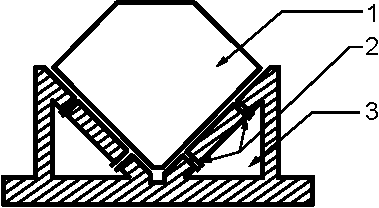
\includegraphics[width=0.5\linewidth]{fyz_fig105.pdf}
      \caption{Příčný řez vzduchovou dráhou: 1 - klouzající předmět; 2 - malé otvory(trysky); 3 -  
               přívod stlačeného vzduchu (\cite[s.~143]{Feynman01})}
      \label{fyz:fig105}
    \end{figure}
    Naše předpoklady o tom, že dva původně nehybné předměty stejných hmotností oddělené explozí 
    odletí na opačné strany stejnými rychlostmi a že dva předměty stejných hmotností stejně rychle 
    proti sobě letící po srážce a splynutí zůstanou nehybné, lze experimentálně prověřit. To je 
    možné provést pozoruhodným zařízením nazývaným vzduchová dráha\footnote{H. V. Neher a R. B. 
    Leighton, Amer. Jour. Of Phys. 31,255 (1963.)}. Toto zařízení nás zbavuje tření, toho tření, 
    které tak trápilo Galilea (obr. \ref{fyz:fig105}). Galileo nemohl provádět experimenty s 
    klouzajícími předměty, neboť neklouzaly dost volně, ale uvedené zařízení nám takové experimenty 
    umožní.

    \begin{figure}[ht!]  %\ref{fyz:fig0106}
      \centering
      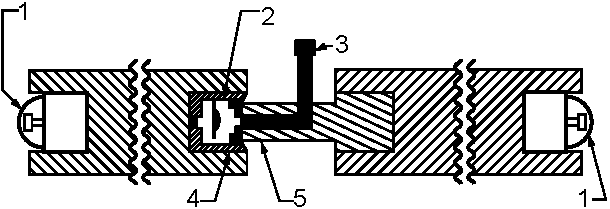
\includegraphics[width=0.7\linewidth]{fyz_fig106.pdf}
      \caption{Podélný řez skluznými bloky spojenými výbušnou náloží: 1 - pružinový amortizátor; 2 - kapsle 
               z dětské pistole; 3 - jiskrová elektroda; 4 - válec; 5 - píst      
                \cite[s.~144]{Feynman01}}
       \label{fyz:fig106}     
    \end{figure}

    \begin{figure}[ht!]  %\ref{fyz:fig107}
      \centering
      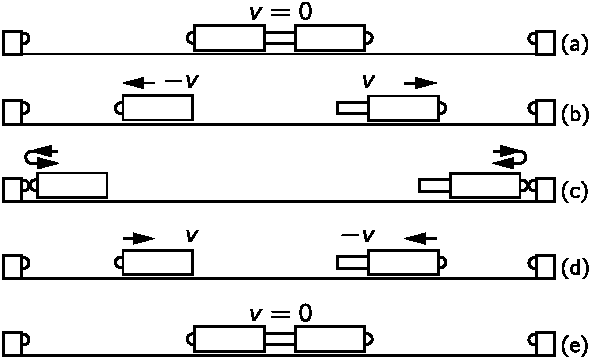
\includegraphics[width=0.7\linewidth]{fyz_fig107.pdf}
      \caption{Schéma experimentu k demonstrace akce a reakce se stejnými hmotnostmi  
               (\cite[s.~144]{Feynman01})}
      \label{fyz:fig107}
    \end{figure}
    Naše předměty budou bez problémů klouzat a ve shodě s Galileovou předpovědí budou mít 
    konstantní rychlost. Dosáhneme toho tak, že předměty se budou pohybovat na vzduchovém polštáři. 
    Protože tření o vzduch je velmi malé, předměty kloužou prakticky konstantní rychlostí, jestliže 
    na ně nepůsobí síla. Nejprve vezmeme dva pečlivě připravené skluzné bloky stejné tíhy a 
    hmotnosti (bloky byly jen zváženy, ale víme, že tíha je úměrná hmotnosti). Mezi tyto bloky 
    vložíme do uzavřeného válce malou výbušnou nálož (obr. \ref{fyz:fig106}). Takto připravené 
    bloky umístíme do středu žlabu a odpálíme nálož elektrickou jiskrou. Co se stane? Jsou-li 
    rychlosti bloků po výbuchu stejné, dosáhnou bloky konce žlabu za stejnou dobu. Po dosažení 
    konců žlabu se bloky odrazí, vrátí se prakticky stejně velkými, ale opačnými rychlostmi 
    do bodu, odkud vycházely a tam se zastaví. To je zajímavý pokus a jeho výsledek je právě 
    takový, jak jsme říkali (obr. \ref{fyz:fig107}).

    \begin{figure}[ht!]  %\ref{fyz:fig108}
      \centering
      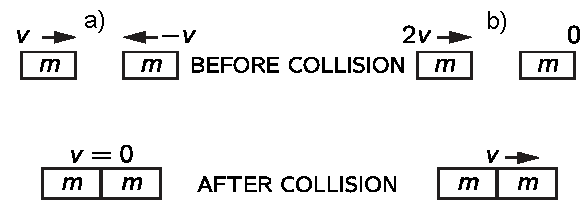
\includegraphics[width=0.7\linewidth]{fyz_fig108.pdf}
      \caption{Dva pohledy na nepružné srážky mezi stejnými hmotnostmi: a) - pohled z těžiště, b) 
               -  pohled z jedoucího auta (rychlost auta \(= -v\))
              (\cite[s.~145]{Feynman01})}
      \label{fyz:fig108}
    \end{figure}
    Dále bychom chtěli ukázat, co se stane ve složitější situaci. Mějme dvě stejné hmotnosti, z 
    nichž jedna se pohybuje rychlostí \(v\) a druhá stojí na místě. Co se s nimi stane, když se 
    srazí a splynou? Po ukončení srážky máme jedno těleso o hmotnosti \(2m\), jež se pohybuje 
    neznámou rychlostí. Zajímáme se o to, jakou. Abychom to zjistili, budeme předpokládat, že se 
    pohybujeme v automobilu podél jejich dráhy. Fyzikální zákony přitom zůstanou stejné, jako 
    kdybychom stáli. Naše úvahy zahájíme poznatkem, že dvě stejné hmotnosti letící proti sobě 
    stejnou rychlostí \(v\) zůstanou po srážce nehybné. Předpokládejme, že po dobu této události 
    jedeme automobilem rychlostí - \(v\). Jak potom vypadá situace? Protože se pohybujeme souběžně 
    s jednou z hmotností, jeví se nám tato tak, jakoby se nepohybovala. Druhá hmotnost, ta, jež se 
    pohybuje rychlostí \(v\) opačným směrem než my, se nám bude jevit tak, jakoby se pohybovala 
    proti nám rychlostí \(2v\) (obr. \ref{fyz:fig108}). Po srážce se spojená hmotnost bude jevit 
    tak, jakoby procházela rychlostí \(v\), nebo, což je matematicky totéž, předmět s rychlostí 
    \(v\) po srážce a splynutí se stejným, původně nehybným předmětem, vytvoří předmět pohybující 
    se rychlostí \(v/2\). Všimněte si, že součet součinů hmotností a rychlostí před srážkou, tj. 
    \(mv + 0\), je stejný jako součet odpovídajících součinů po srážce, tj. \(2mv/2\). Taková je 
    tedy situace, když se těleso letící rychlostí \(v\) srazí s nehybným tělesem.

    Stejným způsobem je možné zjistit, co se stane, když se srazí stejné předměty letící 
    \emph{libovolnými} rychlostmi.

    \begin{figure}[ht!]  %\ref{fyz:fig109}
      \centering
      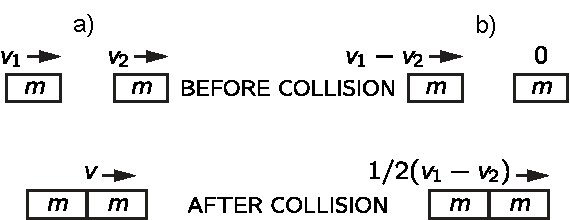
\includegraphics[width=0.7\linewidth]{fyz_fig109.pdf}
      \caption{Dva pohledy na jinou nepružnou srážku mezi dvěma stejnými hmotnostmi: a) - pohled z 
               laboratorního systému, b)- pohled z auta
              (\cite[s.~145]{Feynman01})}
      \label{fyz:fig109}
    \end{figure}
    Předpokládejme, že se srazí a splynou dvě stejná tělesa letící rychlostmi \(v_1\) a \(v_2\). 
    Jaká bude jejich rychlost po srážce? Pojeďme opět automobilem, a to rychlostí \(v_2\), takže 
    jedno z těles se nám bude jevit jako nehybné. Druhé se nám bude jevit tak, jakoby se pohybovalo 
    rychlostí \(v_1 - v_2\) a máme úlohu podobnou té, kterou jsme již uvažovali. Víme, že po srážce 
    se budou tělesa pohybovat rychlostí \(1/2 (v_1 - v_2)\) vzhledem k automobilu. Jaká bude 
    skutečná rychlost těles na zemi? Bude následující: \(v= 1/2(v_1-v_2) + v_2\), tedy \(1/2 (v_1 
    +v_2\) (obr. \ref{fyz:fig108}). Všimněte si, že opět platí
     \begin{equation}\label{fyz:eq141}
      m_1v_1 + m_2v_2 = \frac{2m(v_1 + v_2)}{2}.
    \end{equation}
    
    Použitím tohoto principu můžeme analyzovat libovolnou srážku, při níž se dvě tělesa mající 
    stejné hmotnosti srazí a splynou. Ačkoli jsme ve skutečnosti pracovali jen v jednom rozměru, 
    můžeme se mnoho dozvědět o mnohem složitějších srážkách, když si představíme, že jedeme 
    automobilem v nějakém odkloněném směru. Princip zůstává stejný, jen detaily jsou složitější.

    \begin{figure}[ht!]  %\ref{fyz:fig110}
      \centering
      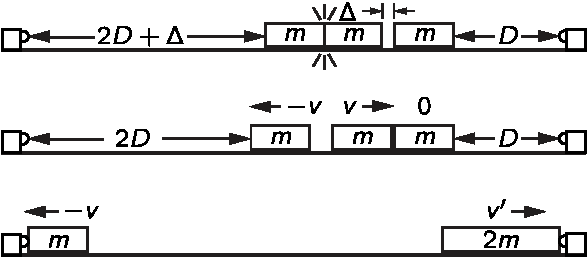
\includegraphics[width=0.7\linewidth]{fyz_fig110.pdf}
      \caption{Experiment k prověření skutečnosti, že hmotnost \(m\) narážející rychlostí \(v\) na hmotnost 
               \(m\) vytváří útvar o hmotnosti \(2m\) a rychlostí \(v/2\)
              (\cite[s.~146]{Feynman01})}
      \label{fyz:fig110}
    \end{figure}
    Abychom experimentálně ověřili, zda předmět letící rychlostí \(v\) vytvoří po srážce se stejným 
    nehybným předmětem předmět pohybující se rychlostí \(v/2\), provedeme na vzduchové dráze 
    následující pokus. Do žlabu umístíme tři předměty se stejnou hmotností, z nichž jsou dva na 
    začátku spojeny již uvedeným explozivním válcem a třetí je sice velmi blízko, ale přece jen 
    oddělený a je na něm přilnavý nárazník, takže se přilepí k předmětu, jenž do něho narazí. V 
    prvním okamžiku po explozi máme dva předměty s hmotností \(m\), které se pohybují v opačném 
    směru stejnými rychlostmi v. V dalším okamžiku se jeden z těchto předmětů sráží s třetím 
    předmětem a vytváří předmět s hmotností \(2m\), jenž by se podle očekávání měl pohybovat 
    rychlostí \(v/2\). Jak se přesvědčíme o tom, že se pohybuje skutečně rychlostí \(v/2\)? 
    Pomůžeme si tak, že počáteční polohy předmětů ve žlabu nastavíme tak, aby vzdálenosti od konců 
    nebyly stejné, ale v poměru \(2:1\). Náš první předmět, který pokračuje v pohybu rychlostí 
    \(v\), by měl projít v dané době dvakrát takovou vzdálenost jako dva předměty, které se spojily 
    (započítáme i malou vzdálenost, již urazí druhý předmět před srážkou s třetím). Hmotnosti \(m\) 
    a \(2m\) by měly dosáhnout konce žlabu současně, a jestliže pokus uskutečníme, zjistíme, že 
    naše očekávání je správné (obr. \ref{fyz:fig109}).

    Dále se budeme zabývat situací, kdy máme dva předměty s různými hmotnostmi. Vezměme hmotnosti 
    \(m\) a \(2m\) a nechme mezi nimi působit naši explozi. Co se pak stane? Jakou rychlostí se 
    pohybuje předmět o hmotnosti \(2m\), jestliže se předmět o hmotnosti \(m\) pohybuje v důsledku 
    exploze rychlostí \(v\)? Experiment, který jsme provedli, můžeme uskutečnit tak, že mezera mezi 
    druhým a třetím předmětem bude nulová a takový pokus nám dá stejný výsledek, tj. hmotnosti 
    \(m\) a \(2m\) dosáhnou rychlosti \(-v\) a \(v/2\). Přímá reakce mezi \(m\) a \(2m\) dává 
    stejný výsledek jako symetrická reakce mezi \(m\) a \(m\), po níž následuje srážka a spojení 
    \(m\) s třetí hmotností \(m\). Dále zjistíme, že hmotnosti \(m\) a \(2m\) se po návratu od 
    konců žlabu s téměř přesně opačnými rychlostmi zastaví, jestliže se spojí.

    Dále se můžeme ptát, co se stane, jestliže předmět o hmotnosti \(m\) letící rychlostí \(v\) 
    narazí na nehybný předmět o hmotnosti \(2m\) a spojí se s ním. Na tuto otázku můžeme odpovědět 
    velmi jednoduše, použijeme-li Galileův princip relativity a srážku, o níž jsme hovořili, 
    pozorujeme z automobilu pohybujícího se rychlostí \(-v/2\) (obr. \ref{fyz:fig111}).

    \begin{figure}[ht!]  %\ref{fyz:fig111}
      \centering
      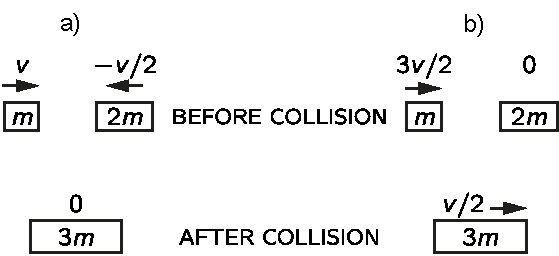
\includegraphics[width=0.7\linewidth]{fyz_fig111.pdf}
      \caption{Dva pohledy na nepružnou srážku mezi hmotnostmi \(m\) a\(2m\): a) - pohled z těžiště 
              systému, b) - pohled z auta)
              (\cite[s.~146]{Feynman01})}
      \label{fyz:fig111}
    \end{figure}
    Při pohledu z automobilu budou rychlosti
    \begin{align*}
      v_1' &= v_1 - v_{\text{auta}} = v + \frac{v}{2} = \frac{3v}{2}   \\
      \shortintertext{a}
      v_2' &= -\frac{v}{2} - v_{\text{auta}} = - \frac{v}{2} + \frac{v}{2} = 0
    \end{align*}
    Po srážce vidíme hmotnost \(3m\) pohybovat se rychlostí \(v/2\). Takto jsme našli odpověď na 
    položenou otázku, tj. poměr rychlostí před srážkou a po srážce je \(3:1\). Sráží-li se předmět 
    o hmotnosti \(m\) s nehybným předmětem o hmotnosti \(2m\) a spojí se s ním, pak se takto 
    vytvořené těleso pohybuje rychlostí, jež je třetinou původní rychlosti. Obecné pravidlo nám 
    opět říká, že součet součinů hmotností a rychlostí zůstává stálý: \(mv + 0\) je rovno \(3m\) 
    krát \(v/3\), a tak kousek po kousku sestavujeme zákon zachování hybnosti.
    
    Zkoumali jsme srážky jednoho tělesa s dvěma tělesy. Použitím stejných argumentů můžeme 
    předpovědět výsledky srážek jednoho tělesa s třemi tělesy, dvou těles s třemi tělesy atd. Obr. 
    \ref{fyz:fig112} znázorňuje případ srážek dvou těles s třemi tělesy a začíná situací, kdy 
    tělesa byla v klidu.
    
    \begin{figure}[ht!]  %\ref{fyz:fig112}
      \centering
      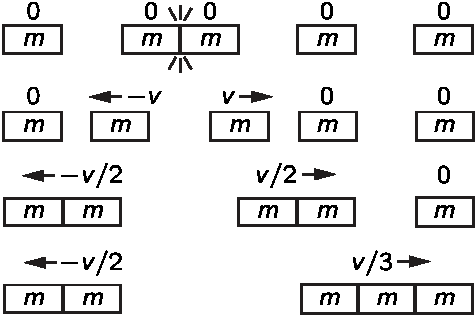
\includegraphics[width=0.6\linewidth]{fyz_fig112.pdf}
      \caption{Akce a reakce mezi tělesy o hmotnostech \(2m\) a \(3m\)
              (\cite[s.~147]{Feynman01})}
      \label{fyz:fig112}
    \end{figure}
    V každém z uvedených případů zjišťujeme, že součin hmotnosti a rychlosti prvního tělesa plus 
    součin hmotnosti a rychlosti druhého tělesa je roven součinu celkové hmotnosti výsledného 
    tělesa a jeho rychlosti. Vše jsou to tedy příklady na zákon zachování hybnosti. Vycházeli jsme 
    z jednoduchých, symetrických případů a poukázali na platnost tohoto zákona v složitějších 
    případech. Tak lze postupovat v případě libovolného racionálního poměru hmotností, a protože 
    každé číslo lze s libovolnou přesností vyjádřit pomocí racionálního čísla, náš postup bude 
    možno uplatnit libovolně přesně pro jakýkoli poměr hmotností.
     
  \section{Hybnost a energie}
    Všechny předcházející příklady byly jednoduché v tom smyslu, že dvě tělesa se po srážce 
    spojila, nebo byla spojena a později oddělena explozí. Existují však případy, kdy se tělesa 
    nespojí, jako např. dvě tělesa se stejnými hmotnostmi, jež vstupují do srážky se stejnými 
    absolutními hodnotami rychlostí a po srážce se rozletí na různé strany. V kratičkém okamžiku 
    jsou v kontaktu a obě se stlačí. V okamžiku největšího stlačení mají obě dvě nulovou rychlost a 
    energie je uchována v těchto pružných tělesech tak jako ve stlačené pružině. Tato energie 
    pochází z kinetické energie, již měla tělesa před srážkou, a jež se stává nulovou, je-li 
    rychlost nulová. Ztráta kinetické energie však trvá jen okamžik. Stlačení se podobá náloži, 
    která uvolňuje energii při explozi. Ihned nastává dekomprese podobná explozi a tělesa se 
    opět rozletí. Tento případ však již známe - tělesa odletí stejnými rychlostmi. Obecně je však 
    rychlost po  odrazu menší než počáteční rychlost, neboť ne všechna energie se využije k odrazu. 
    Záleží na materiálu, jaká část energie se využije k odrazu. Je-li materiál plastický, neuvolní 
    se žádná kinetická energie, ale je-li materiál pružný, určitá část kinetické energie se uvolní. 
    Při srážce se zbytek kinetické energie přemění v tepelnou a kmitavou energii - tělesa se 
    zahřejí a kmitají. Později se i energie kmitů přemění v teplo. Srážející se tělesa je možno 
    konstruovat z velmi pružného materiálu, jakým je například ocel, a při pečlivé volbě 
    pružinových nárazníků je možné dosáhnout toho, že při srážce vzniká jen velmi málo tepla a 
    kmitů. V takovýchto podmínkách jsou rychlosti odrazu prakticky rovné počátečním rychlostem a 
    takové srážky nazýváme \textbf{pružnými}.
    
    Skutečnost, že rychlosti \emph{před} pružnou srážkou a po ní jsou stejné, není důsledkem zákona 
    zachování hybnosti, ale důsledkem zachování \emph{kinetické energie}. To, že rychlosti těles 
    odrážejících se po symetrické srážce \emph{jsou stejné}, je však důsledkem zákona zachování 
    hybnosti.
    
    Podobným způsobem můžeme analyzovat srážky mezi tělesy, která mají různé hmotnosti, počáteční 
    rychlosti i stupně pružnosti, a určit výsledné rychlosti a ztrátu kinetické energie, ale těmito 
    podrobnostmi se již nebudeme zabývat.
    
    Pružné srážky jsou zvlášť zajímavé v systémech, které nemají vnitřní „kolečka, ozubená kola 
    nebo jiné části“. V takových systémech nemá energie při srážkách kam unikat, neboť odrážející 
    se objekty se nacházejí ve stejných podmínkách jako před srážkou. Proto se mezi elementárními 
    objekty uskutečňují pružné nebo téměř pružné srážky. Například srážky mezi atomy nebo 
    molekulami plynu jsou považovány za dokonale pružné. Ačkoli tu jde o výbornou aproximaci, ani v 
    takovémto případě nejsou srážky \emph{dokonale} pružné - jinak si nemůžeme vysvětit, odkud bere 
    plyn energii na světelné a tepelné záření. Občas se při srážkách v plynu emituje 
    nízkoenergetické infračervené záření. Jeho výskyt je však velmi ojedinělý a emitovaná energie 
    je velmi malá. Srážky molekul v plynech je proto většinou možno považovat za dokonale pružné.
    
    Všimněme si zajímavého příkladu \emph{pružných} srážek mezi dvěma tělesy se \emph{stejnými 
    hmotnostmi}. Přibližují-li se takováto tělesa k sobě stejně velkými rychlostmi, pak se z důvodů 
    symetrie budou od sebe vzdalovat stejnými rychlostmi. Podívejme se však na tento proces v jiné 
    situaci, kdy jedno z nich se pohybuje rychlostí \(v\) a druhé je v klidu. Co se stane? S něčím 
    podobným jsme se již setkali. Symetrickou srážku budeme pozorovat z auta pohybujícího se 
    souběžně s jedním z těles a zjistíme, že pohybující se těleso při pružné srážce s nehybným 
    tělesem stejné hmotnosti zastaví, a to, které bylo v klidu, se bude pohybovat stejnou rychlostí 
    jako první těleso. Tělesa si prostě vymění rychlosti\footnote{Tento výsledek poprvé publikoval 
    český fyzik Jan Marek Marci v roce 1639.}. Takové chování lze snadno ověřit vhodným srážkovým 
    zařízením. Obecně, pohybují-li se obě tělesa proti sobě různými rychlostmi, prostě si při 
    srážce rychlosti vymění. Jiným příkladem téměř pružných interakcí je magnetizmus. Umístíme-li 
    dvojici podkovovitých magnetů na naše kluzné bloky tak, že se vzájemně odpuzují, pak při 
    opatrném posunutí jednoho směrem k druhému dojde k odtlačení druhého magnetu, první magnet se 
    úplně zastaví a druhý se pak bude bez tření pohybovat.
    
    Zákon zachování hybnosti je velmi užitečný a umožňuje nám vyřešit mnoho problémů bez jejich 
    podrobného zkoumání. Neznali jsme detailně pohyb plynu při výbuchu nálože, a přece jsme 
    například dokázali předpovědět rychlosti, s jakými se tělesa odrazí. Dalším zajímavým příkladem 
    je raketový motor. Raketa s velkou hmotností \(M\) vymršťuje malé množství plynů hmotnosti 
    \(m\), ale obrovskou rychlostí \(V\) vzhledem k samotné raketě. Původně nehybná raketa se proto 
    začne pohybovat malou rychlostí \(v\). Pomocí zákona zachování hybnosti můžeme tuto rychlost 
    vypočítat, a tak dostaneme
    \begin{equation}\label{fyz:eq142}
      v = \frac{m}{M}\cdot V.
    \end{equation}
    Pokud je plyn vymršťován, raketa nabírá rychlost. Raketový pohon je v podstatě totéž, co zpětný 
    náraz pušky; nepotřebuje vzduch k tomu, aby se od něho odrážel.
    
  \section{Relativistická hybnost}
    Není to tak dávno, co zákon zachování hybnosti postihly určité změny. Samotný zákon sice stále 
    platí, ale změny nastaly v definici. V \emph{teorii relativity} se ukazuje, že zákon zachování 
    hybnosti platí. Částice mají hmotnost, a hybnost je definována opět jako součin hmotnosti a 
    rychlosti, tj. \(mv\), jenže hmotnost se v závislosti na rychlosti mění, a proto se bude měnit 
    i hybnost. Změna hmotnosti podléhá zákonu
    \begin{equation}\label{fyz:eq143}
      m = \dfrac{m_0}{\sqrt{1 - \dfrac{v^2}{c^2}}}.
    \end{equation}
    kde \(m_0\) je hmotnost tělesa v \emph{klidu}, \(c\) je rychlost světla. Z tohoto vztahuje 
    zřejmé, že \(m\) se jen nepatrně liší od \(m_0\), pokud v není velmi velká, a tak pro běžné 
    rychlosti je možné vyjádřit hybnost starým vztahem.
    
    Složky hybností jedné částice lze zapsat ve tvaru
    \begin{equation}\label{fyz:eq144}
      p_x = \dfrac{m_0v_x}{\sqrt{1 - \dfrac{v^2}{c^2}}}, \quad
      p_y = \dfrac{m_0v_y}{\sqrt{1 - \dfrac{v^2}{c^2}}}, \quad
      p_z = \dfrac{m_0v_z}{\sqrt{1 - \dfrac{v^2}{c^2}}},
    \end{equation}
    přičemž \(v^2 = v_x^2 + v_y^2 + v_z^2\). Sečteme-li \(x\)-ové složky všech interagujících 
    částic nejprve před srážkou a pak po srážce, zjistíme, že tyto součty jsou stejné, tj. hybnost 
    ve směru osy \(x\) se zachovává. Totéž platí v libovolném směru.
    
    V kapitole \ref{fyz:IchapII} jsme viděli, že zákon zachování energie neplatí, nepřipustíme-li 
    existenci různých forem energie: elektrické, mechanické, tepelné, zářivé apod. V některých z 
    těchto případů (např. u tepelné energie) je možno říci, že energie se vyskytuje v „skryté“ 
    formě. Tento příklad nás může inspirovat k otázce: „Existují i skryté formy hybnosti - 
    například tepelná hybnost?“  Odpověď na tuto otázku je, že hybnost se dá velmi obtížně skrýt, a 
    to z následujících důvodů.
    
    Součet druhých mocnin rychlostí neuspořádaně se pohybujících atomů tělesa představuje míru 
    tepelné energie. Jako výsledek dostaneme kladnou veličinu bez směrového charakteru. Teplo 
    existuje bez ohledu na to, zda se těleso jako celek pohybuje, nebo zda je nehybné, a zachování 
    energie v podobě tepla není přímo zřejmé. Dostaneme-li však při sčítání \emph{rychlostí}, které 
    mají směr, výsledek různý od nuly, znamená to, že existuje pohyb samotného tělesa v jistém 
    směru, a ten již můžeme viditelně pozorovat. Neexistuje tedy náhodná, uvnitř utajená hybnost; 
    těleso má nenulovou hybnost jen tehdy, když se pohybuje jako celek. Proto lze hybnost jako 
    mechanickou veličinu těžko skrýt. Hybnost je však přece jenom \emph{možné} skrýt - např. v 
    elektromagnetickém poli. To je další zvláštnost teorie relativity.
    
    Newton předpokládal, že vzájemné působení se bez ohledu na vzdálenost uskutečňuje okamžitě. 
    Tento předpoklad se ukázal být nesprávným. Uvažujeme-li například i elektrické síly a v určitém 
    místě uvedeme do pohybu elektrický náboj, pak se jeho vliv na jiný náboj v jiném místě 
    neprojeví okamžitě - existuje malé zpoždění. V takovéto situaci i při rovnosti sil akce a 
    reakce se hybnosti nebudou kompenzovat; bude existovat krátký časový interval, v jehož průběhu 
    nastanou problémy. V této době pocítí první náboj určitou sílu reakce a získá určitou hybnost, 
    zatímco druhý náboj ještě nepocítil nic a jeho hybnost se nezměnila. Vzájemné působení 
    potřebuje k překlenutí vzdálenosti určitou dobu, takovou, jako kdyby se šířilo rychlostí 
    \SI{300000}{\km\per\s}. V průběhu takovéhoto kraťoučkého intervalu se hybnost částic 
    nezachovává. Pocítí-li však druhý náboj působení prvního náboje a vše se ustálí, zákon 
    zachování hybnosti bude opět platit; nezachovává se tedy jen po krátkou dobu. Záhadný je tedy 
    jen ten krátký časový interval. Situaci si představujeme tak, že v tomto intervalu existuje i 
    jiná hybnost, než je hybnost částic \(mv\). Jde o hybnost elektromagnetického pole. Přidáme-li 
    tuto hybnost pole k hybnosti částic, pak se hybnost zachovává v kterémkoli okamžiku. To, že 
    elektromagnetické pole může mít hybnost a energii, ho činí skutečné reálným, a tak původní 
    myšlenku o existenci sil mezi částicemi je třeba pozměnit v tom smyslu, že částice vytváří pole 
    a pole působí na jinou částici. Samotné pole má dobře známé vlastnosti jako jsou energie a 
    hybnost, vlastnosti, které mají částice. Jako další příklad si všimněme elektromagnetického 
    pole, v němž existují vlny nazývané světlem. Ukazuje se, že světlo má i hybnost, a proto při 
    dopadu na předmět přináší i určité množství hybnost. To je ale rovnocenné působení síly, neboť 
    získává-li osvětlený předmět určité množství hybností za sekundu, jeho hybnost se mění a 
    situace je stejná, jako kdyby na něj působila síla. Při dopadu na předmět vyvolává světlo tlak. 
    Tento tlak je velmi malý, ale dostatečně citlivými zařízeními ho můžeme změřit.
   
    V kvantové mechanice se ukazuje, že hybnost je něco jiného - už to není \(mv\). Je těžké přesně 
    definovat, co je to rychlost částice, ale hybnost přece existuje. V kvantové mechanice je 
    rozdíl v tom, že když se částice chovají jako částice, je hybnost \(mv\), ale když se chovají 
    jako vlny, měří se hybnost počtem vln najeden metr: Čím větší je počet vln, tím větší je 
    hybnost. Bez ohledu na tyto rozdíly platí zákon zachování hybnosti i v kvantové mechanice. 
    Ačkoli zákon \(f= ma\) v kvantové mechanice neplatí a Newtonovo odvození zákona zachování 
    hybností je nesprávné, přece jen v kvantové mechanice samotný zákon zachování hybnosti platí!
    
    
  \section{Příklady a cvičení}
  
%} %tikzset
%---------------------------------------------------------------------------------------------------